\section{Genetic Programming}
\emph{Genetic Programming} (GP) is a class of search algorithms for finding optimal programs based on the principle of natural evolution first proposed by John Koza~\cite{koza1994genetic}.
In general, a program $p$ can be considered as a mapping from the set of inputs $\mathcal{I}$ to the corresponding set of outputs $\mathcal{O}$
\begin{equation}
	p : \mathcal{I} \to \mathcal{O}.
\end{equation}
However, since not all input-output pairs are known in advance, this mapping is usually given in form of a finite set of training cases.
The goal of GP is then to find a program that correctly computes the correct output for each input contained in the training set.
Since there is often not a unique program that satisfies this condition, usually a number of additional constraints are applied to assess the quality of each correct program.
For instance, in practice one is often interested in finding the shortest or fastest program that is able to pass all training cases.
Based on a program's effectiveness in solving all training cases under the given constraints, GP then assigns a \emph{fitness} value to each program, which is then treated as an \emph{individual} within a \emph{population} of programs.
In evolutionary computation, the population is a set of individuals currently considered within the search and, therefore, spans a subspace within the space of solutions for the given search problem.
Each subsequent step of the search is then performed by generating a new population based on the previous one through \emph{mutation} or recombination (often called \emph{crossover}) of the individuals contained in the current one.
Usually, the candidates for mutation and crossover are sampled from the current population based on the fitness value computed for each individual.
If we repeat this procedure for a number of $n$ steps, we arrive at a final population $P_n$, which can then additionally be evaluated on a test set, to obtain the best overall program.
The resulting search method is summarized in Algorithm~\ref{alg:genetic-programming}. 
\begin{algorithm}[t]
	\caption{Genetic Programming}
	\label{alg:genetic-programming}
	\begin{algorithmic} % The number tells where the line numbering should start
		\State \textbf{Randomly generate} an initial population $P_0$ of programs
		\State \textbf{Evaluate} $P_0$ on the \textbf{training set} 
		\For{$i := 1, \dots, n$}
		\State \textbf{Select} a subset of individuals $M_i \supset P_{i-1}$ based on their \textbf{fitness}
		\State \textbf{Generate} new programs $C_i$ based on $M_i$ using \textbf{mutation} and \textbf{crossover}
		\State \textbf{Evaluate} $C_i$ on the \textbf{training set} 
		\State \textbf{Select} $P_{i}$ from $C_i \cup P_{i-1}$
		\EndFor
		\State \textbf{Evaluate} the final population $P_{n}$ on a \textbf{test set}  to obtain the best overall program
	\end{algorithmic}
\end{algorithm}
While Algorithm~\ref{alg:genetic-programming} gives an overview of the general structure of a GP method, we have not yet considered how the individual operations such as the generation of an initial population and the creation of new individuals through mutation and crossover can be performed.
Since all these operations are based on manipulating the internal structure of a given program, the first step in the implementation of a GP method choosing a suitable program representation.
Note that this representation does not necessarily need to be equal to the target language in which the actual program is supposed to be implemented but rather needs to define a unique mapping that enables its automatic generation.
This process is usually called \emph{genotype} to \emph{phenotype} mapping, where the genotype refers to the internal representation used within GP while the phenotype then represents the actual program implemented on the target machine.
One of the most widely used genotype representations is tree-based GP, where each program is internally represented as a tree of expressions, which was also initially proposed by John Koza~\cite{koza1994genetic}.
While within the last decades numerous other GP variants have been proposed~\cite{poli2008field}, such as grammatical evolution~\cite{o2001grammatical}, linear GP~\cite{brameier2007linear} and cartesian GP~\cite{miller2008cartesian}, we focus on tree-based GP as it forms the basis for our implementation, which will be presented in later chapters.
\section{Representation}
In contrast to other evolutionary algorithms algorithms, which usually represent the solution to an optimization problem as an array of discrete or continuous numbers~\cite{back1997handbook}, GP deals with the optimization of programs and, hence, each solution corresponds to an executable program.
%Before we consider these operations in detail, we first need to define a procedure to generate program expression trees in a structured way. 
For this purpose, we consider the following context-free grammar $G$ with the productions
\begin{equation}
	\begin{split}
		S & \to E \\
		E & \to \text{if} \; B \; \text{then} \; E \; \text{else} \; E \; | \; A \\
		A & \to -A \; | \; (A + A) \; | \; (A - A) \; | \; (A \cdot A) \; | \; A^A \; | \; x \; | \; y \\  
		B & \to \neg B \; | \; (B \wedge B) \; | \; (B \vee B) \; | \; u \; | \; v,
	\end{split}
\label{eq:gp-example-grammar}
\end{equation}
where $V = \{S, E, A, B\}$ is the set of variables and the symbols $x$, $y$ represent numbers while the symbols $u$, $v$ correspond to boolean values, i.e. $\top$ or $\bot$.
If we treat $x$, $y$, $u$ and $v$ as an input, each expression generated by $G$ can be considered as a quaternary function $f(x,y,u,v) \in L_{G}$, where $L_G$ is the language generated by $G$ according to Definition~\ref{def:language}.
For example the functions
\begin{equation}
	\begin{split}
		f_1(x,y,u,v) & = \text{if} \; (\neg u \wedge v) \; \text{then} \; (x \cdot x) \; \text{else} \; (x / y) \\
		f_2(x,y,u,v) & = x^{(x + y)} - (y \cdot y)
	\end{split}
\label{eq:gp-example-functions}
\end{equation} can both be generated by $G$ and are, hence, included in $L_G$.
By applying the rules of arithmetic and boolean algebra, we can compute the result of each such function based on a given set of inputs.
Therefore, assuming both $x$ and $y$ represent real-valued numbers, we can evaluate the correctness of the mapping $f : x, y, u, v \to \mathbb{R}$ for an arbitrary number of test cases.
Next, to define suitable operations for generating arbitrary functions $f \in L_G$, we need to choose a suitable data structure for its representation.
While a program's structure depends on the programming language it is formulated in, in many cases it is possible to formulate it as a tree of program expressions, which is especially true for languages from the Lisp-family, that have been originally employed in John Koza's work~\cite{koza1994genetic}.
In tree-based GP all operations are performed on program expression trees and, thus, both mutation and crossover must be designed with respect to this representation.
Expression trees can be created in a straightforward way after rewriting each expression in postfix notation. 
To obtain the corresponding tree, the expressions is traversed sequentially by putting each operand that either represents a terminal symbol or has been already transformed on a stack and then retrieving those operands from the top of the stack for each new operator encountered.
Figure~\ref{fig:gp-expression-tree-examples} shows the corresponding expression trees for $f_1$ and $f_2$.
\begin{figure}
	\begin{subfigure}{0.59\textwidth}
		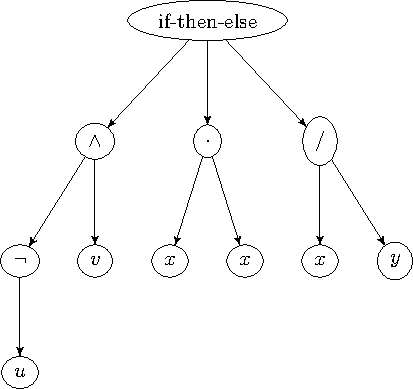
\includegraphics{figures/gp_expression_tree1.pdf}
	\end{subfigure}
	\begin{subfigure}{0.41\textwidth}
		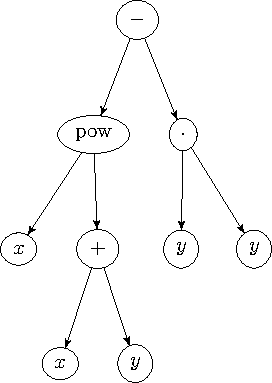
\includegraphics{figures/gp_expression_tree2.pdf}
	\end{subfigure}
 \caption{Expression trees for $f_1$ and $f_2$, where we have simplified the if-then-else construct to a single ternary operator.}
 \label{fig:gp-expression-tree-examples}
\end{figure}
On the other hand, given a certain expression tree, we can easily restore the original expression by traversing the tree recursively in a top-down manner while generating the corresponding expression for each node as soon as each of its operands has been recursively processed or in case it is available as a terminal symbol.
While expression trees can be both easily generated from a given program, as well as offering an efficient way to evaluate a certain program, they possess an inherent limitation, which is the absence of type information.
For a better understanding of this, we reconsider the context-free grammar formulated in Equation~\eqref{eq:gp-example-grammar}.
Therein all productions on the variable $B$ only result in the generation of boolean expressions, while all productions starting from $A$ exclusively lead to arithmetic expressions.
As a consequence, we are not allowed to intermix expressions that are derived from $A$ and $B$.
However, this information is not contained in any of the expressions generated by $G$ and, hence, also missing in the corresponding tree.
As the generation of each new expression can be performed based on the productions of $G$, it is guaranteed to be valid.
However, the main step of GP is the creation of new individuals based on the existing ones in the population either through recombination of two individuals (crossover) or by altering certain parts of a given individual (mutation). 
Both operations require us to investigate which nodes and subtrees of a given expression trees can be safely replaced by an alternative branch without violating the type constraints imposed within the productions of our grammar.
While it is possible to deal with this problem by simply evicting those individuals that violate any type constraints from the population, depending on the number of constraints, this will be the case for a high percentage of individuals, leading to a highly inefficient method.
A different and usually more efficient approach is to annotate each node within an expression tree with additional type information, which leads to the concept of strongly-typed GP, first proposed by David Montana~\cite{montana1995strongly}.
Strongly-typed GP represents a viable solution to the problem of retaining type correctness, but it requires us to transform the implicit type information contained within the productions of our grammar into explicit type annotations at the nodes of each expression tree.
As an alternative we can instead utilize the information encoded in the productions of a grammar $G$ by considering the \emph{derivations} of an expression $e \in L_G$, as defined by
\begin{equation}
	S \Rightarrow e_1 \Rightarrow e_2 \Rightarrow \dots \Rightarrow e_n \Rightarrow e.
\end{equation}
If $G$ is context-free each of its possible derivations can be represented as a tree, where the root node is always the start variable $S$ and each vertex of the tree corresponds to a transition between sequential forms within the derivation~\cite{linz2006introduction}.
More formally we can define a derivation tree as follows:
\begin{definition}[Derivation Tree]\label{def:derivation-tree}
	Let $G = \left\{V, T, S, P\right\}$ be a context-free grammar, then a derivation tree is an ordered tree with the following properties
\begin{enumerate}
	\item The start variable $S$ is the root of the tree.
	\item If $a$ is a leaf then $a \in T \cup \{\lambda \}$.
	\item If $A$ is an interior node then $A \in V$.
	\item If $A$ is an interior node and its children are $a_1, a_2, \dots, a_n$, then $P$ must contain a production of the form
	\begin{equation}
		A \to a_1 a_2 \dots a_n.
	\end{equation}  
\end{enumerate}
\end{definition} 
%Furthermore, if $G$ is regular, its derivations can be further simplified to finite state machine, where each state corresponds to a sequential form.
Consider again the grammar whose productions are shown in Equation~\eqref{eq:gp-example-grammar} and the example functions $f_1$ and $f_2$ as defined in Equation~\eqref{eq:gp-example-functions}.
Based on these productions, we can formulate derivations that lead to the expressions of both functions, for example 
\begin{equation}
\begin{aligned}
	\bm{S} & \Rightarrow \bm E \Rightarrow \bm A \Rightarrow A - A \Rightarrow A^A - \bm A \Rightarrow A^{\bm A} - (A \cdot A) \Rightarrow \bm{A}^{A + A} - (A \cdot A) \\  
	& \Rightarrow x^{\bm A + A} - (A \cdot A) \Rightarrow x^{x + \bm A} - (A \cdot A) \Rightarrow x^{x + y} - (\bm A \cdot A) \\ 
	& \Rightarrow x^{x + y} - (y \cdot \bm A) \Rightarrow x^{x + y} - (y \cdot y) = f_2(x,y,u,v)
\end{aligned}
\end{equation}
represents a valid derivation for $f_2$, where each variable that is transformed next is written in bold font.

